% Template by Shuai Wang @ ILLC, UvA

\documentclass[12pt]{article}
\usepackage[utf8]{inputenc}
\usepackage[T1]{fontenc}
\usepackage{graphicx}
\usepackage{xcolor}
\usepackage{pgfplots}
\usepackage{hyperref}
\usepackage{listings} 
% \usepackage[utf8]{inputenc}
\usepackage[english]{babel}
\usepackage[]{algorithm2e}
 \usepackage{listings}
\usepackage{amsthm}

\usepackage{multirow}
% \usepackage[]{algorithm2e}
\usepackage{ amssymb }

\theoremstyle{definition}
\newtheorem{definition}{Definition}[section]
 
\usepackage{cite}

\usepackage{multirow}

\usepackage{ amssymb }
\usepackage[]{algorithm2e}

\usepackage{parcolumns}
\usepackage{lipsum}
\usepackage{url}
\urldef{\mailsa}\path|{alfred.hofmann, ursula.barth, ingrid.haas, frank.holzwarth,|
\urldef{\mailsb}\path|anna.kramer, leonie.kunz, christine.reiss, nicole.sator,|
\urldef{\mailsc}\path|erika.siebert-cole, peter.strasser, lncs}@springer.com|    
\newcommand{\keywords}[1]{\par\addvspace\baselineskip
\noindent\keywordname\enspace\ignorespaces#1}


\newtheorem{theorem}{Theorem}[section]
\newtheorem{corollary}{Corollary}[theorem]
\newtheorem{lemma}[theorem]{Lemma}

% \theoremstyle{definition}
% \newtheorem{definition}{Definition}[section]
 
\include{defs}

%%%%%%%%%%%%%%%
% Title Page
\title{Title}
\author{Shuai Wang \newline Supervisor : XXXX
\newline Course       : Dynamic Epistemic Logic \newline ILLC, UvA }
\date{\today}
%%%%%%%%%%%%%%%

\begin{document}
\maketitle

\tableofcontents
\clearpage

% \section{Features commands}

% \subsection{Pictures used}

% \noindent
% Cover picture filename (in titlepage): \texttt{cover}\\
% Logo filename (in foot): \texttt{logo}

% \subsection{Boxes}

% \begin{verbatim}
% \fullboxbegin
% Content
% \fullboxend
% \end{verbatim}

% \begin{verbatim}
% \leftboxbegin
% Content
% \leftboxend
% \end{verbatim}

% \begin{verbatim}
% \rightboxbegin
% Content
% \rightboxend
% \end{verbatim}

% \begin{verbatim}
% \frameboxbegin{Frame Title}
% Content
% \frameboxend
% \end{verbatim}


\section*{Abstract}
% This project is as a part of the course \textbf{Dynamic Epistemic Logic} by ILLC, UvA. This project aims at exploring the implementation of propositional epistemic learning functions and extending BDI Agent Framework with epistemic learning features. 
I am an abstract.
% % \keywords{action learning, epistemic learning, scalable learning algorithms}
% \end{abstract}

\newpage

% \section{First section}
% \lipsum[1]

% \fullboxbegin
% \lipsum[1]
% \fullboxend

% \lipsum[1]
\section{Project Proposal}
 
 
 I am a project proposal. The following is a plot. 



\begin{figure}[!ht]
\centering
\caption{Scalability Evaluation - Average Time}
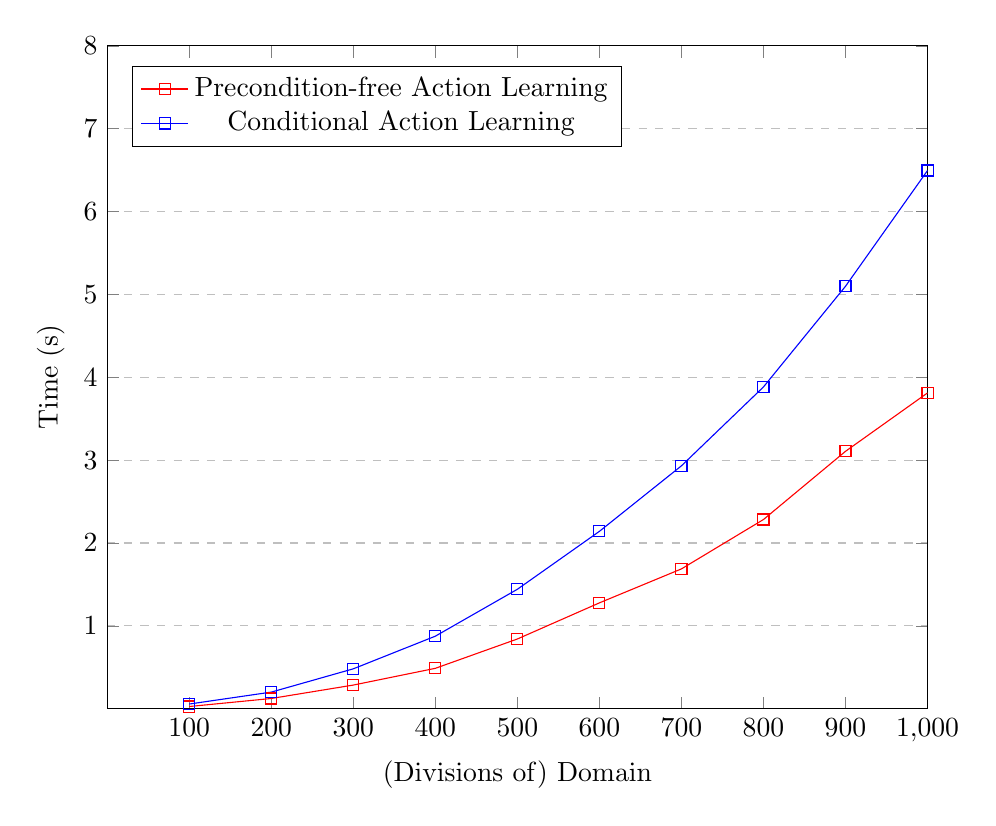
\begin{tikzpicture}
\label{fig5}
\begin{axis}[
    % title={Precondition Free Action Learning - Average Time},
    xlabel={(Divisions of) Domain},
    ylabel={Time (s)},
    xmin=0, xmax=1000,
    ymin=0, ymax= 8.0,
    xtick={100,200,300,400, 500, 600, 700, 800, 900, 1000},
    ytick={1.0,  2.0,  3.0,  4.0,  5.0,  6.0, 7.0, 8.0},
    legend pos=north west,
    ymajorgrids=true,
    grid style=dashed,
    width=12cm, height=10cm
]
    \addplot[
    color=red,
    mark=square,
    ]
    coordinates {
(100 , 0.026) 
(200 , 0.123) 
(300 , 0.285) 
(400 , 0.487) 
(500 , 0.841) 
(600 , 1.277) 
(700 , 1.687) 
(800 , 2.283) 
(900 , 3.106) 
(1000 , 3.811) 

    };
    \addlegendentry{Precondition-free Action Learning} 
    
    
\addplot[
    color=blue,
    mark=square,
    ]
    coordinates {
(100 , 0.056) 
(200 , 0.200) 
(300 , 0.481) 
(400 , 0.875) 
(500 , 1.441) 
(600 , 2.140) 
(700 , 2.931) 
(800 , 3.883) 
(900 , 5.098) 
(1000 , 6.495) 
    };
    \addlegendentry{Conditional Action Learning}
    %  \addlegendentry{\#Pre=20}

 
\end{axis}
\end{tikzpicture}
\end{figure}



\begin{figure}[!ht]
\centering
\caption{Scalability Evaluation - Average \#Observation}
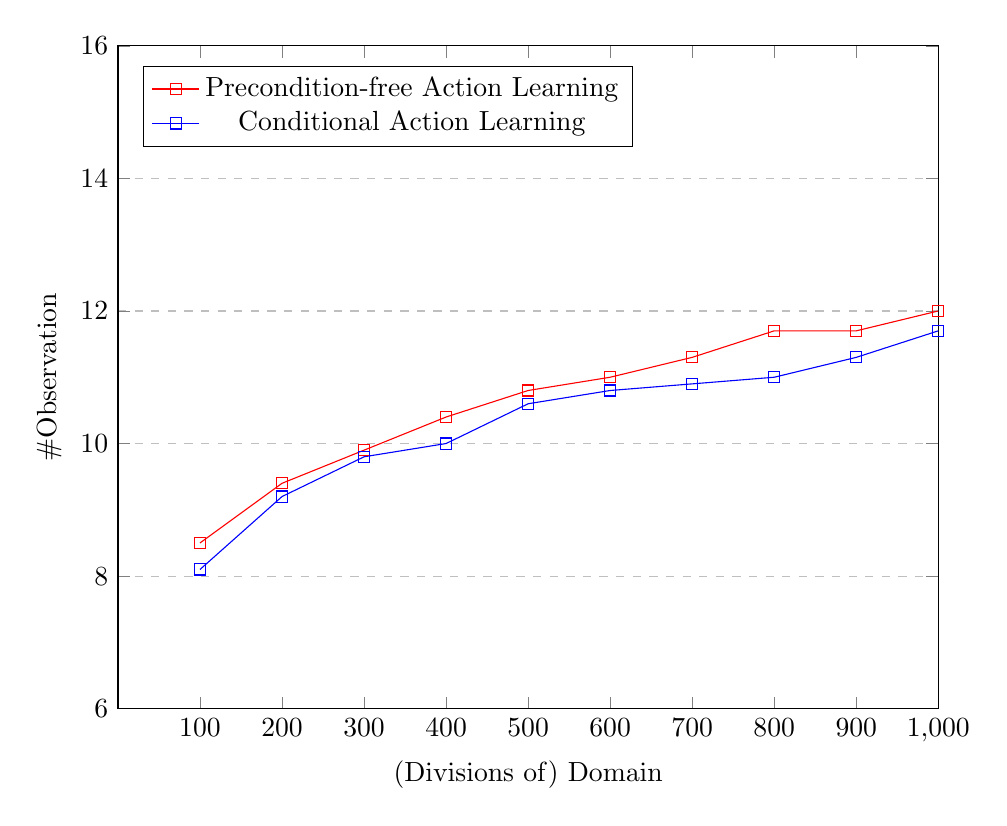
\begin{tikzpicture}
\label{fig6}
\begin{axis}[
    % title={Precondition Free Action Learning - Average Time},
    xlabel={(Divisions of) Domain},
    ylabel={\#Observation},
    xmin=0, xmax=1000,
    ymin=6, ymax=16,
    xtick={100,200,300,400, 500, 600, 700, 800, 900, 1000},
    ytick={6,8,10,12,14,16},
    legend pos=north west,
    ymajorgrids=true,
    grid style=dashed,
    width=12cm, height=10cm
]
  
\addplot[
    color=red,
    mark=square,
    ]
    coordinates {
(100 , 8.5
)(200 , 9.4
)(300 , 9.9
)(400 , 10.4
)(500 , 10.8
)(600 , 11.0
)(700 , 11.3
)(800 , 11.7
)(900 , 11.7
)(1000 , 12.0
)

    };
    \addlegendentry{Precondition-free Action Learning}
    
\addplot[
    color=blue,
    mark=square,
    ]
    coordinates {
(100 , 8.1)
(200 , 9.2)
(300 , 9.8)
(400 , 10.0)
(500 , 10.6)
(600 , 10.8)
(700 , 10.9)
(800 , 11.0)
(900 , 11.3)
(1000 , 11.7)

    };
    \addlegendentry{Conditional Action Learning}

    
\end{axis}
\end{tikzpicture}
\end{figure}





\begin{figure}[!ht]
\centering
\caption{\#Pre-\#Post Correspondence - Average Time}
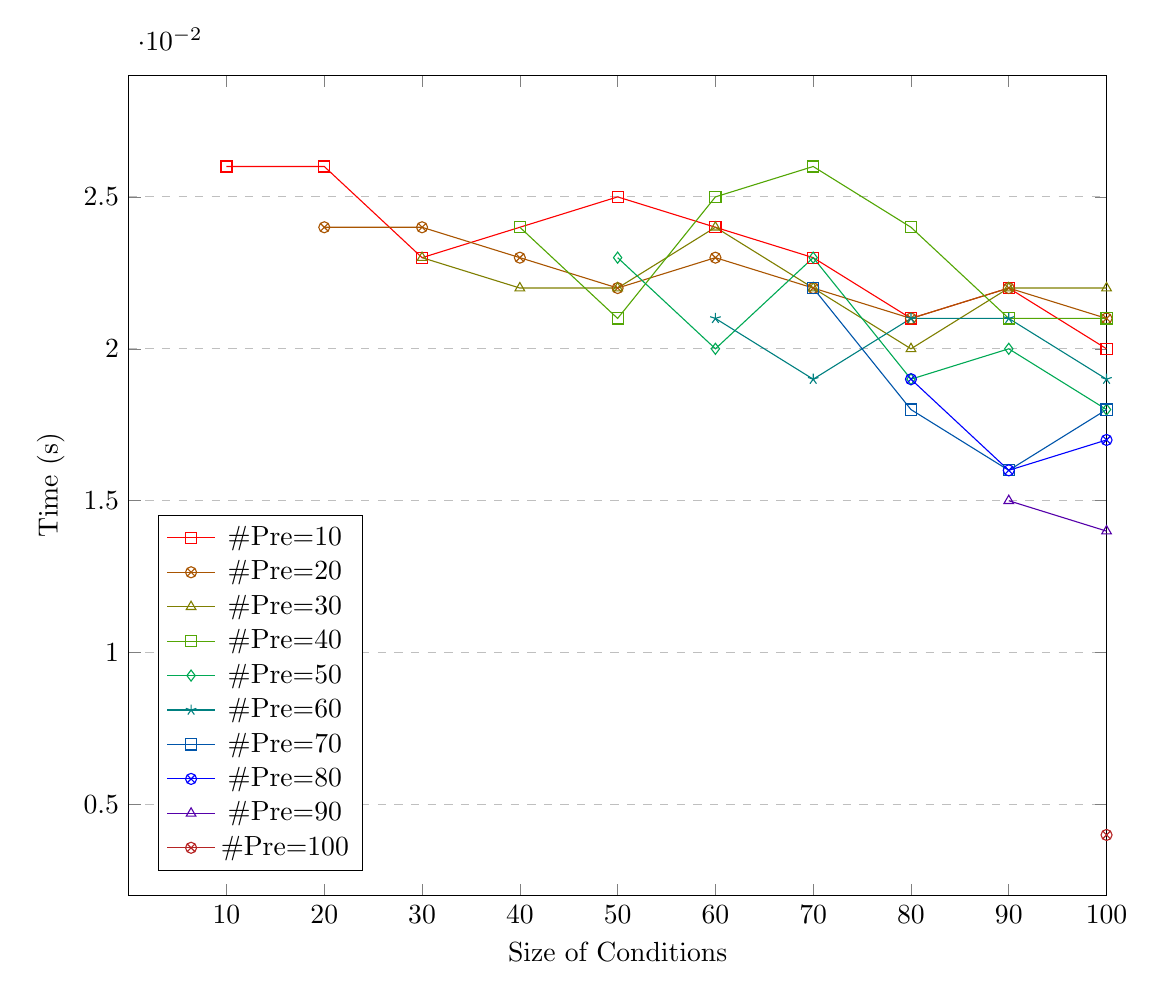
\begin{tikzpicture}[]
\label{fign}
\begin{axis}[
    % title={Precondition Free Action Learning - Average Time},
    xlabel={Size of Conditions},
    ylabel={Time (s)},
    xmin=0, xmax=100,
    ymin=0.002, ymax=0.029,
    xtick={10,20,30,40, 50, 60, 70, 80, 90, 100},
    ytick={0.005, 0.010, 0.015, 0.020, 0.025},
    legend pos=south west,
    ymajorgrids=true,
    grid style=dashed,
    width=14cm, height=12cm
]
 
\addplot[
    color={rgb:red,255;green,1;blue,1},
    mark=square,
    ]
    coordinates {
(10 , 0.026)
(20 , 0.026)
(30 , 0.023)
(40 , 0.024)
(50 , 0.025)
(60 , 0.024)
(70 , 0.023)
(80 , 0.021)
(90 , 0.022)
(100, 0.020)
    };
 \addlegendentry{\#Pre=10}

        
\addplot[
    color={rgb:red,255;green,128;blue,1},
    mark=otimes,
    ]
    coordinates {
(20 , 0.024)
(30 , 0.024)
(40 , 0.023)
(50 , 0.022)
(60 , 0.023)
(70 , 0.022)
(80 , 0.021)
(90 , 0.022)
(100, 0.021)
    };
 \addlegendentry{\#Pre=20}
 
 \addplot[
    color={rgb:red,255;green,255;blue,1},
    mark=triangle,
    ]
    coordinates {
(30 , 0.023)
(40 , 0.022)
(50 , 0.022)
(60 , 0.024)
(70 , 0.022)
(80 , 0.020)
(90 , 0.022)
(100, 0.022)
    };
 \addlegendentry{\#Pre=30}
 
 
 \addplot[
    color={rgb:red,128;green,255;blue,8},
    mark=square,
    ]
    coordinates {
(40 , 0.024)
(50 , 0.021)
(60 , 0.025)
(70 , 0.026)
(80 , 0.024)
(90 , 0.021)
(100, 0.021)
    };
 \addlegendentry{\#Pre=40}
 
  \addplot[
    color={rgb:red,1;green,255;blue,128},
    mark=diamond,
    ]
    coordinates {
(50 , 0.023)
(60 , 0.020)
(70 , 0.023)
(80 , 0.019)
(90 , 0.020)
(100, 0.018)
    };
 \addlegendentry{\#Pre=50}
 
   \addplot[
    color={rgb:red,0;green,255;blue,255},
    mark=star,
    ]
    coordinates {
% (50 , 0.0252)
(60 , 0.021)
(70 , 0.019)
(80 , 0.021)
(90 , 0.021)
(100, 0.019)
    };
 \addlegendentry{\#Pre=60}
 
  
   \addplot[
    color={rgb:red,0;green,128;blue,255},
    mark=square,
    ]
    coordinates {
% (50 , 0.0252)
% (60 , 0.0220)
(70 , 0.022)
(80 , 0.018)
(90 , 0.016)
(100, 0.018)
    };
 \addlegendentry{\#Pre=70}
 
 
 
   \addplot[
    color={rgb:red,0;green,0;blue,255},
    mark=otimes,
    ]
    coordinates {
% (50 , 0.0252)
% (60 , 0.0220)
% (70 , 0.0231)
(80 , 0.019)
(90 , 0.016)
(100, 0.017)
    };
 \addlegendentry{\#Pre=80}
 
 
  
   \addplot[
    color={rgb:red,127;green,0;blue,255},
    mark=triangle,
    ]
    coordinates {
% (50 , 0.0252)
% (60 , 0.0220)
% (70 , 0.0231)
% (80 , 0.0184)
(90 , 0.015)
(100, 0.014)
    };
 \addlegendentry{\#Pre=90}
 
    \addplot[
    color={rgb:red,5;green,1;blue,1},
    mark=otimes,
    ]
    coordinates {
% (50 , 0.0252)
% (60 , 0.0220)
% (70 , 0.0231)
% (80 , 0.0184)
% (90 , 0.0162)
(100, 0.004)
    };
 \addlegendentry{\#Pre=100}
 
 
 
 
\end{axis}
\end{tikzpicture}
\end{figure}




\begin{figure}[!ht]
\centering
\caption{\#Pre-\#Post Correspondence - Average \#Observation}
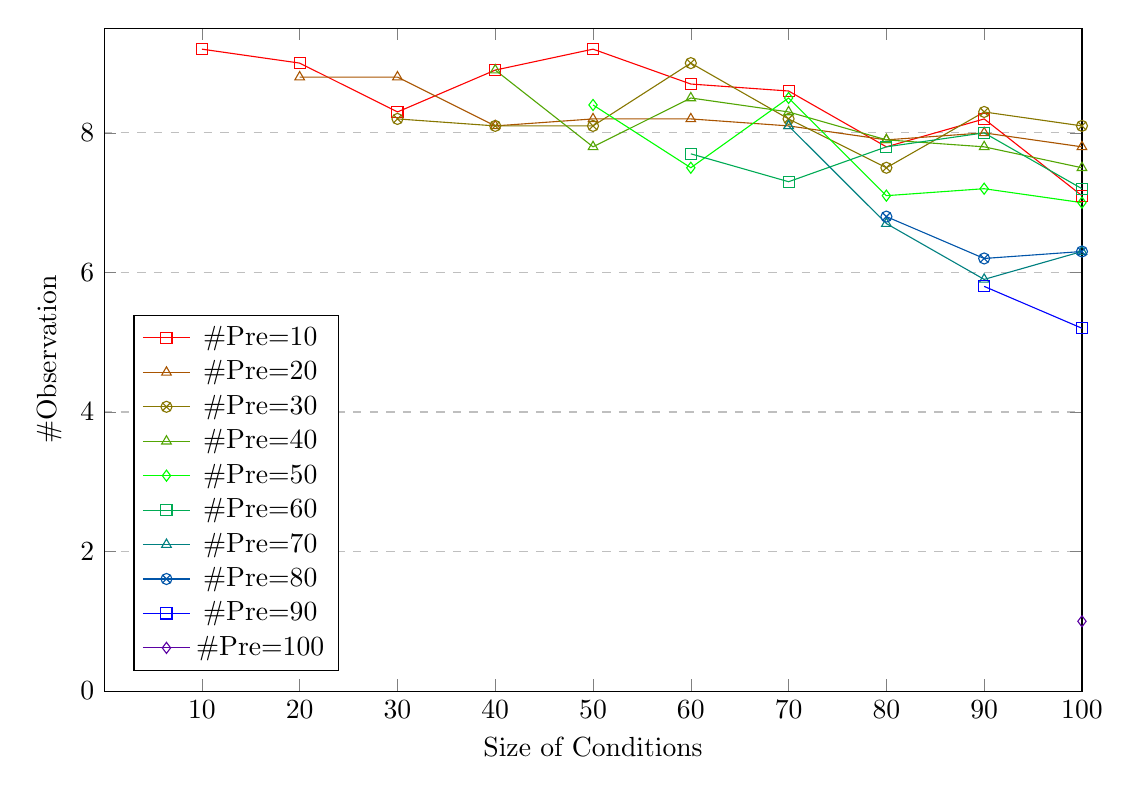
\begin{tikzpicture}[]
\label{fignn}
\begin{axis}[
    % title={Precondition Free Action Learning - Average Time},
    xlabel={Size of Conditions},
    ylabel={\#Observation},
    xmin=0, xmax=100,
    ymin=0.000, ymax=9.5,
    xtick={10,20,30,40, 50, 60, 70, 80, 90, 100},
    ytick={0, 2, 4, 6, 8, 10},
    legend pos=south west,
    ymajorgrids=true,
    grid style=dashed,
    width=14cm, height=10cm
]
 
\addplot[
    color={rgb:red,255;green,1;blue,1},
    mark=square,
    ]
    coordinates {
(10 , 9.2)
(20 , 9.0)
(30 , 8.3)
(40 , 8.9)
(50 , 9.2)
(60 , 8.7)
(70 , 8.6)
(80 , 7.8)
(90 , 8.2)
(100, 7.1)
    };
 \addlegendentry{\#Pre=10}

    \addplot[
    color={rgb:red,255;green,128;blue,1},
    mark=triangle,
    ]
    coordinates {
% (10 , )
(20 , 8.8)
(30 , 8.8)
(40 , 8.1)
(50 , 8.2)
(60 , 8.2)
(70 , 8.1)
(80 , 7.9)
(90 , 8.0)
(100, 7.8)
    };
 \addlegendentry{\#Pre=20}

\addplot[
    color={rgb:red,255;green,225;blue,1},
    mark=otimes,
    ]
    coordinates {
% (10 , 8)
% (20 , 8)
(30 , 8.2)
(40 , 8.1)
(50 , 8.1)
(60 , 9.0)
(70 , 8.2)
(80 , 7.5)
(90 , 8.3)
(100, 8.1)
    };
 \addlegendentry{\#Pre=30}

\addplot[
    color={rgb:red,128;green,255;blue,8},
    mark=triangle,
    ]
    coordinates {
% (10 , )
% (20 , )
% (30 , )
(40 , 8.9)
(50 , 7.8)
(60 , 8.5)
(70 , 8.3)
(80 , 7.9)
(90 , 7.8)
(100, 7.5)
    };
 \addlegendentry{\#Pre=40}

\addplot[
    color={rgb:red,0;green,250;blue,0},
    mark=diamond,
    ]
    coordinates {
% (10 , )
% (20 , )
% (30 , )
% (40 , )
(50 , 8.4)
(60 , 7.5)
(70 , 8.5)
(80 , 7.1)
(90 , 7.2)
(100, 7.0)
    };
 \addlegendentry{\#Pre=50}

\addplot[
    color={rgb:red,0;green,255;blue,125},
    mark=square,
    ]
    coordinates {
% (10 , )
% (20 , )
% (30 , )
% (40 , )
% (50 , )
(60 , 7.7)
(70 , 7.3)
(80 , 7.8)
(90 , 8.0)
(100, 7.2)
    };
 \addlegendentry{\#Pre=60}

\addplot[
    color={rgb:red,0;green,255;blue,255},
    mark=triangle,
    ]
    coordinates {
% (10 , )
% (20 , )
% (30 , )
% (40 , )
% (50 , )
% (60 , )
(70 , 8.1)
(80 , 6.7)
(90 , 5.9)
(100, 6.3)
    };
 \addlegendentry{\#Pre=70}

\addplot[
    color={rgb:red,1;green,128;blue,255},
    mark=otimes,
    ]
    coordinates {
% (10 , )
% (20 , )
% (30 , )
% (40 , )
% (50 , )
% (60 , )
% (70 , )
(80 , 6.8)
(90 , 6.2)
(100, 6.3)
    };
 \addlegendentry{\#Pre=80}

\addplot[
    color={rgb:red,0;green,1;blue,255},
    mark=square,
    ]
    coordinates {
% (10 , )
% (20 , )
% (30 , )
% (40 , )
% (50 , )
% (60 , )
% (70 , )
% (80 , )
(90 , 5.8)
(100, 5.2)
    };
 \addlegendentry{\#Pre=90}

\addplot[
    color={rgb:red,125;green,1;blue,225},
    mark=diamond,
    ]
    coordinates {
% (10 , )
% (20 , )
% (30 , )
% (40 , )
% (50 , )
% (60 , )
% (70 , )
% (80 , )
% (90 , 5)
(100, 1)
    };
 \addlegendentry{\#Pre=100}

 
 
\end{axis}
\end{tikzpicture}
\end{figure}







\bibliography{thesis}
\bibliographystyle{plain}

\end{document}     


% \lstset{language=Haskell}
% \begin{lstlisting}[frame=single, basicstyle=\footnotesize]
% \end{lstlisting}